\documentclass[12pt,english]{article}
\usepackage[utf8]{inputenc}
\usepackage[a4paper]{geometry}
\geometry{verbose,tmargin=2cm,bmargin=2cm,lmargin=3cm,rmargin=2cm,headheight=12pt,headsep=24pt}
\setcounter{secnumdepth}{4}
\usepackage{titlesec}
\titleformat{\paragraph}
{\normalfont\normalsize\bfseries}{\theparagraph}{1em}{}
\titlespacing*{\paragraph}
{0pt}{3.25ex plus 1ex minus .2ex}{1.5ex plus .2ex}
\setcounter{tocdepth}{3}
\usepackage{pdfpages}
\usepackage{bm}
\usepackage{array}
\usepackage{float}
\usepackage{graphicx}
\usepackage{tocloft}
\usepackage{hyperref}
\hypersetup{
    colorlinks=true,
    linkcolor=blue,
    filecolor=blue,      
    urlcolor=blue,
}
\usepackage{setspace}
\PassOptionsToPackage{normalem}{ulem}
\usepackage{ulem}
\usepackage{indentfirst}	%Az összes címsor utáni bekezdést beljebb viszi%
\usepackage{amsmath}
\usepackage{tikz}
\usepackage{wrapfig}
\usetikzlibrary{shadings}

\usepackage{pgfplots}


\usepackage{hyperref}
\hypersetup{
    colorlinks,
    citecolor=black,
    filecolor=black,
    linkcolor=black,
    urlcolor=black
}




\makeatletter

%%%%%%%%%%%%%%%%%%%%%%%%%%%%%% LyX specific LaTeX commands.
\newcommand{\noun}[1]{\textsc{#1}}
%% Because html converters don't know tabularnewline
\providecommand{\tabularnewline}{\\}

%%%%%%%%%%%%%%%%%%%%%%%%%%%%%% Textclass specific LaTeX commands.
\newenvironment{lyxcode}
{\par\begin{list}{}{
\setlength{\rightmargin}{\leftmargin}
\setlength{\listparindent}{0pt}% needed for AMS classes
\raggedright
\setlength{\itemsep}{0pt}
\setlength{\parsep}{0pt}
\normalfont\ttfamily}%
 \item[]}
{\end{list}}

%%%%%%%%%%%%%%%%%%%%%%%%%%%%%% User specified LaTeX commands.
%\textwidth 160mm
%\oddsidemargin 0cm
%\topmargin -15mm
\usepackage{bm}
\newcommand{\tg}{\mathop\mathrm{tg}}
\newcommand{\grad}{\mathop\mathrm{grad}}
\newcommand{\BME}{\hrule\vspace{6pt}{\large Budapest University of Technology and Economics
\\
Faculty of Mechanical Engineering \\
Department of Applied Mechanics}}
\newcommand{\szerzo}{}
\newcommand{\konzulensek}{
\parbox[t]{20cm}
{\normalsize
\hspace*{25em} Made by:\\
\hspace*{28em}Bálint CSATÓ\\
\hspace*{25em}Supervisor:\\
\hspace*{28em}Gergely GYEBRÓSZKI \\
}\hfill}

\makeatother

\usepackage{babel}


\begin{document}



\title{\vspace{-2cm}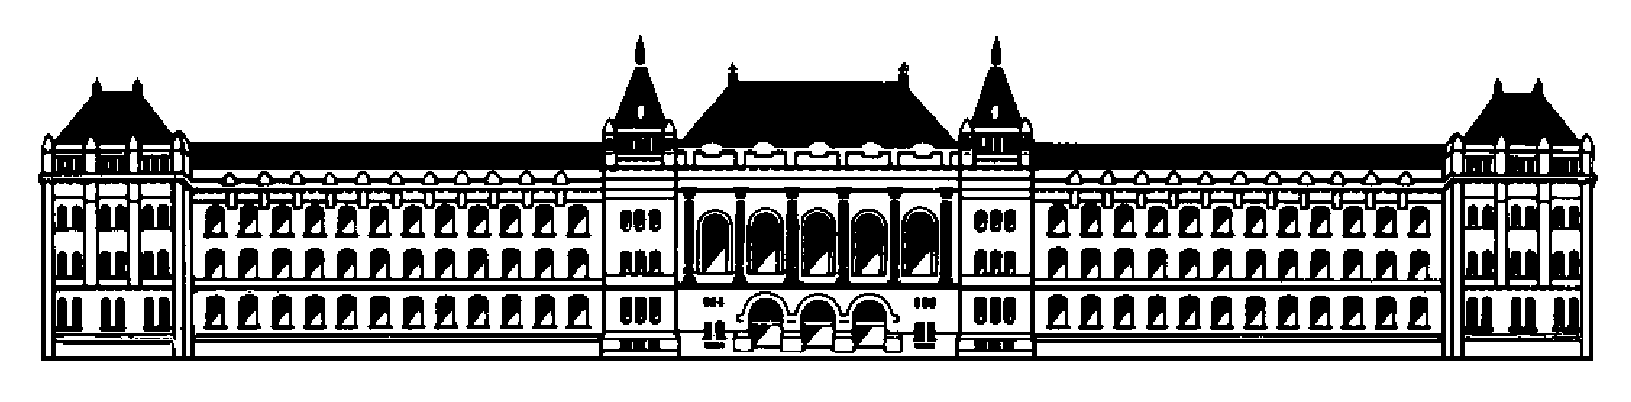
\includegraphics[width=0.4\textwidth,keepaspectratio]{figures/bme_skyline}\\
\BME\vspace{4cm}\\
Control and Parameter Estimation Problems of Autonomous Transport Robots
\\[5mm]
\large{Final Project}}


\author{\sc\szerzo}


\date{\vspace{6cm}\konzulensek\\
\vspace{3cm}Budapest, 2018}

\maketitle
\thispagestyle{empty}



\newpage
\pagenumbering{arabic}
\renewcommand{\contentsname}{Contents}
\renewcommand{\cftsecleader}{\cftdotfill{\cftdotsep}}
\tableofcontents
\numberwithin{equation}{section} % Number equations within sections
\numberwithin{figure}{section} % Number figures within sections
\numberwithin{table}{section} % Number tables within sections

\newpage
%%%%%%%%%%%%%%%%%%%%%%%%%%%%%%%%%%%%%%%%%%%%%%%%%%%%%%%%%%%%%%%%%%%%%%%%%%%%%%%%%%%%%%%%%%%%%%%%%%%%%%%%%%%%
% 													Preface
%%%%%%%%%%%%%%%%%%%%%%%%%%%%%%%%%%%%%%%%%%%%%%%%%%%%%%%%%%%%%%%%%%%%%%%%%%%%%%%%%%%%%%%%%%%%%%%%%%%%%%%%%%%%
\section*{Preface}
Autonomous vehicle technology offers the possibility of fundamentally
changing transportation. Equipping cars and light vehicles
with this technology will likely reduce crashes, energy consumption,
and pollution and reduce the costs of congestion, as well.............
blabalblablalblalba
lablblablablalblballb
labllablblalbalblalblbal

\addcontentsline{toc}{section}{Preface}

\newpage
%%%%%%%%%%%%%%%%%%%%%%%%%%%%%%%%%%%%%%%%%%%%%%%%%%%%%%%%%%%%%%%%%%%%%%%%%%%%%%%%%%%%%%%%%%%%%%%%%%%%%%%%%%%%
% 											Introduction to Autonomous Transport Robots
%%%%%%%%%%%%%%%%%%%%%%%%%%%%%%%%%%%%%%%%%%%%%%%%%%%%%%%%%%%%%%%%%%%%%%%%%%%%%%%%%%%%%%%%%%%%%%%%%%%%%%%%%%%%
\section{Introduction to Autonomous Transport Robots}
\subsection{History of transportation}

Since the early days of the human civilization, one of the most common problem has been the transportation. The first major development was the domestication of animals what made it possible to transport more and heavier loads or humans themselves in order to achieve greater speed and duration. The next substantial invention was the wheel which increased the efficiency of animal transport introducing the concept of vehicles. Until the Industrial Revolution, the water transport facilities proved to be the most effective way. With the development of the combustion engines and automobiles around the end of the 19st century, road transport became competitive again. Today trucks transport cargos over thousands of miles, but light items are still being carried in wheelbarrows or trailers attached to more compact vehicles. 

\begin{figure}[h]
	\centering
	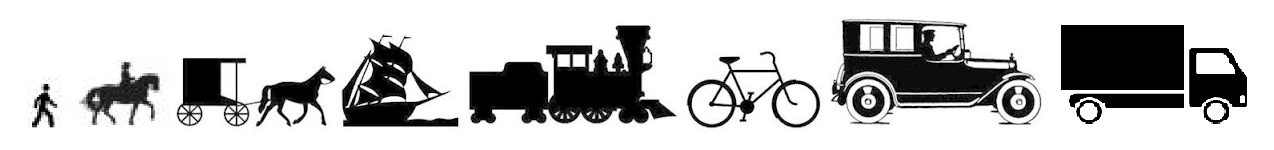
\includegraphics[width=10cm]{figures/evot}
	\label{fig1}
	\caption{Evolution of Transportation}
\end{figure}

\noindent One of the most dominant development tendency in almost every field of the industry is the automation of processes and procedures. Automation means the reduction of human intervention in the operation of machines. The benefit of automation include labor savings, savings in electricity costs, savings in material costs, and improvements to quality, accuracy and precision. The most trending application of the automation regarding the transportation is the autonomous cars on the roads. 
\subsection{Autonomous vehicles}
An autonomous car which is also known as a self-driving car or a driverless car, is a vehicle that can operate without a certain amount of human control using its sensors to monitor the informations coming from the environment. Great variety of techniques are used to detect the surroundings, such as radar, laser light, GPS, odometry and computer vision. The collected information provides a decent input to the control system which is the soul of the self-driving cars. Several control problems have to be solved continuously during driving on the roads, such as identifying obstacles and avoiding them, following transportation rules or navigating along a predefined path.

Autonomous vehicle technology offers the possibility of fundamentally
changing transportation. Equipping cars and light vehicles
with this technology will likely reduce traffic collisions, thus the resulting injuries and the related costs including less need for insurance. Autonomous cars are predicted to increase the traffic flow and the mobility of citizens. Reduced traffic congestion and the improvements in traffic flow due to widespread use of autonomous cars will also translate into better fuel efficiency and reduced pollution in cities.

In spite of the various benefits also several issues exist such as technology challenges, disputes concerning liability, customer concerns about the safety of driverless cars, risk of loss of privacy and security concerns against hackers, risk of negative effects on the society and economy and finally moral issues when car's software is forced to choose between multiple harmful alternatives during an inevitable accident. 
 

The autonomous driving technology can be most easily conceptualized using a five-part
continuum suggested by the National Highway Traffic Safety Administration
(NHTSA), with different benefits of the technology realized
at different levels of automation:
\begin{itemize}
	\item \textbf{Level 0:}  The human driver is in complete control of all functions of the car.
	\item \textbf{Level 1:}  One function is automated.
	\item \textbf{Level 2:}  More than one function is automated at the same time (e.g., steering and acceleration), but the driver must remain constantly attentive.
	\item \textbf{Level 3:} The driving functions are sufficiently automated that the driver can safely engage in other activities.
	\item \textbf{Level 4:} The car can drive itself without a human driver.\cite{c}
\end{itemize}
\noindent

From engineering point of view, the most important issues are the technological challenges, i.e. how to design a driverless vehicle system which is capable of handling vehicle's performance like human in all possible conditions. An autonomous vehicle is a combination of sensors and actuators, sophisticated algorithms executed as a software on a processor.
The sensory system can be classified into three different classes:
\begin{itemize}
	\item \textbf{Navigation and guidance:} the system which determines – where you are, where you want to go, and how do you get there. In the most common applications different techniques such as GPS, compass and dead reckoning are used.
	\item \textbf{Driving and Safety:} Directing the vehicle and making sure that vehicle follows the rules of the road. The autonomous car must be able to see and interpret what is in front of it when it is going forward (and behind when in reverse). It is also necessary to see what is on either side, in other words, it needs a 360$^{\circ}$ view. A set of video cameras is an obvious choice by which location of lanes and surrounding objects or markers on the road can determined.
	\item \textbf{Performance:} managing car's internal system. Several application specific, unique circuit boards and subsystems are added to a conventional vehicle to provide the functions needed for autonomous operation. Much of the system-level operation involves measuring and managing the power requirements to control power, overall consumption, and thermal dissipation.
\end{itemize}

The concept of driverless cars made a lot of attention over the past ten years. Generally speaking it can be said that one of the most determining development directions in the automotive industry are related to automated solutions. Many people still do not believe that there could be such a possibility with fully driverless vehicles due to the fact that there so many parameters in the driving function that have to be controlled simultaneously and continuously and even a single failure could cause catastrophy. Nowadays after a lot of research and experiments self-driving cars can be seen as a reality, or at least close future. Still, there are many challenges in designing a fully autonomous system for a self-driving car. The challenges of driverless cars can be sorted into five groups:

\begin{itemize}
	\item  \textbf{Road conditions:} 
	Road conditions can be unpredictable and varying, i.e. in some cases they are smooth and well-marked while in other cases there are no lane marking. On some roads there can be potholes, in case of mountainous and tunnel roads the visibility of external signals for direction are poor.
	
	\item 	\textbf{Weather conditions:}
	It can be sunny and clear or rainy and stormy weather. Autonomous cars have to work in all weather conditions, there is no scope for any failure.
	
	\item \textbf{Traffic conditions:}
	Maybe this is the most complex problem as the human behaviour and autonomous car algorithm have to be matched with each other. The cars would have to drive in all sorts of traffic conditions as humans can do it. The people are emotional beings operating irrationally sometimes. Beside the fact that the traffic would be highly self-regulated, in certain cases some people might break the rules resulting an unpredictable situation in point of a self-driving car. An object may turn up in an unexpected conditions, e.g. crashed car which have to be bypassed ignoring some traffic rules. It can be handled by humans easily but for an artificial intelligence it is a harder task as its operation is ruled by rule-following conditions and this kind of situation needs the capability of detecting the need to ignore the rules in that specific case. The lack of intelligence of several autonomous cars on the roads could result in traffic deadlock.
	
	\item \textbf{Accident Liability:}
	One of the most important aspect of autonomous cars is accidents liability. Who is liable for accidents caused by a self-driving car?
	Generally, the software will be the main component that will drive the car and will make all the good and bad decisions. At initial levels of design there is a person who is physically behind the steering wheel and can take over the control, but in newer designs does not have even any dashboard, pedals and steering wheel. In such cars the driver, who is actually almost just a passenger cannot be the liable for an accident. Furthermore, due to the nature of autonomous cars, the drivers can be supposed to be in a relaxed state without paying sufficient attention to handle unexpected traffic conditions, thus by the time they need to act, it may be too late.
	
	\item \textbf{Radar Interference:}
	Autonomous cars use lasers and radar for navigation. The principle of radar works by detecting reflections of radio waves from surrounding objects. The time taken for the reflection is measured to calculate the distance between the car and the object and appropriate action is then taken based on the radar readings. The problems will come up when thousands of cars on the roads try to use the technology because the reflected radar signals can interfere making it difficult to distinguish which signal was emitted by which vehicle. Even if choosing a different radio frequency can eliminate the issue, the available frequency range is unlikely to be sufficient for all the vehicles manufactured.
	\cite{5c}
\end{itemize}
As a conclusion it can be stated that there are still lot of challenges beside the fact that there have been already some autonomous cars on the roads nowadays, but mostly for development and research purposes. Probably, the collective effort of the industry will definitely make the autonomous car in everyday life a reality one day because the benefits are considered to be remarkable. The most important expected benefit would be the reduction of losses of live in road accidents. Benefits with secondary importance are the reduction of fuel consumption, therefore the environment pollution caused by the vehicles, furthermore time and cost savings could be realized due to optimized behaviour. Time, cost and energy savings are top wanted purposes in almost every field of industry and everyday life, therefore autonomous solutions with such desired features will likely appear in more and more applications. 

\subsection{Application of autonomous transport robots}
The conventional ways of transporting could be appropriate for most of the cases but not in those when repeated passages to specific locations in small distances have to be taken.
One of the latest trends in technology is to create such driverless robots that can help people in their everyday life, i.e. bringing any kind of products to customers. A company called Starship launched a several self-driving robotic vehicles on the streets of Washington, D.C. that can transport food and other small items to customers ordering via app.
\begin{figure}[h]
	\centering
	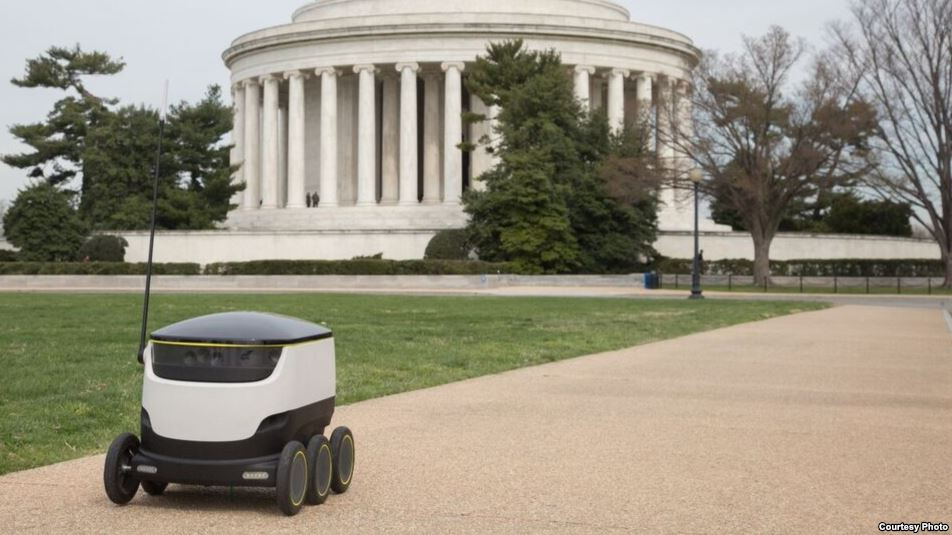
\includegraphics[width=7cm]{figures/starship.jpg}
	\label{fig1}
	\caption{Starship Technologies}
\end{figure}
The robotic vehicles move themeselves along sidewalks using camera and tracking technology to avoid any obstacle and its location can be tracked from the distance in order to know the time of arrival. The six-wheeled electric machine sits about a half-meter high having a lockable cargo bay to carry food products up to nine kilograms in weight.\cite{starship}




A company called SMP Robotics made automated guided vehicles that can remove grass clippings and fallen leaves or construct garbage collection in a garden. 
\begin{figure}[h]
	\centering
	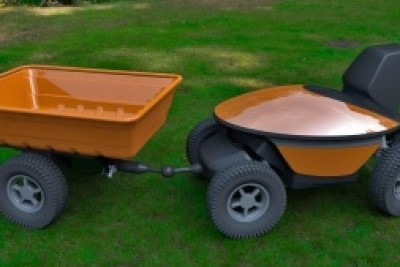
\includegraphics[width=7cm]{figures/smp.jpg}
	\label{smp}
	\caption{SMP Robotics}
\end{figure}

\noindent These small-sized mobile robots have a trailer attached to the back. They are powered by electrical engines, thus noise and smell emission is minimized which allow for operation around people. The built-in accumulators stores the needed energy and can last for several days of cyclical operation. Two ways of route following method is available. The first option is to choose a root in advance with the help of the attached PC tablet. The second way is to set the robot in its 'follow me' algorithm whereby it is going to follow the operator and learn the path. The collected goods on the trailer can be unloaded automatically using a mechanism without any human intervention. The trailer can be fitted with a water tank which can be used for watering of grass and other plants, furthermore automatic water refill algorithm is implemented. This kind of automatic self-moving watering system suits really well such occasions when a fixed irrigation systems are not worth being built due to climate characteristics.\cite{smp}

A firm named NEOBOTIX made autonomous transport system for daily use in industrial applications. The robots are equipped with laser scanners that permanently detect landmarks and obstacles what allows the robot to react dynamically to unexpected changes of their surrounding, i.e. to safely operate between human and other moving objects. This flexibility makes them suited for dynamic transportation tasks with frequent changes. For instance, they can complement roller or belt conveyors and take parts to machines or workplaces that are not connected to the conveyor system. \cite{neo}

\begin{figure}[htb!]
	\centering
	\minipage{0.50\textwidth}
	\centering
	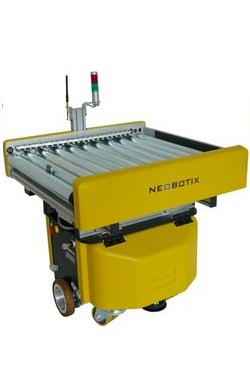
\includegraphics[height=5cm]{figures/neo1.jpg}
	\caption{{\small MT-400}}
	\endminipage\hfill
	\minipage{0.50\textwidth}
	\centering
	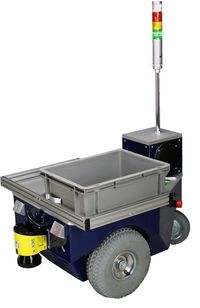
\includegraphics[height=5cm]{figures/neo2.jpg}
	\caption{{\small MT-500}}
	\label{conv2}
	\endminipage\hfill
\end{figure} 

\noindent Possible applications are taking parts to and from workplaces, transporting in direct interaction with humans or dynamic picking of parts for later assembly

BMW logistics also uses autonomous transport robots similarly in industrial environment. The well-known car manufacturer has been working hard to reduce emissions in all steps of the manufacturing process of a car, not only in the final product. This application shows really well that the autonomous developments in the automotive industry is not just about the autonomous driving on the roads but the manufacturing processes as well. Smart Transport Robots (STR) transport components through logistics at the Wackersdorf plant. They measures the distance to wireless transmitters which are located at in the logistics hall to calculate its exact position and route. Using sensors to identify and react to critical situations, it is able to share the route with humans and other vehicles. \cite{bmw}

\begin{figure}[htb!]
	\centering
	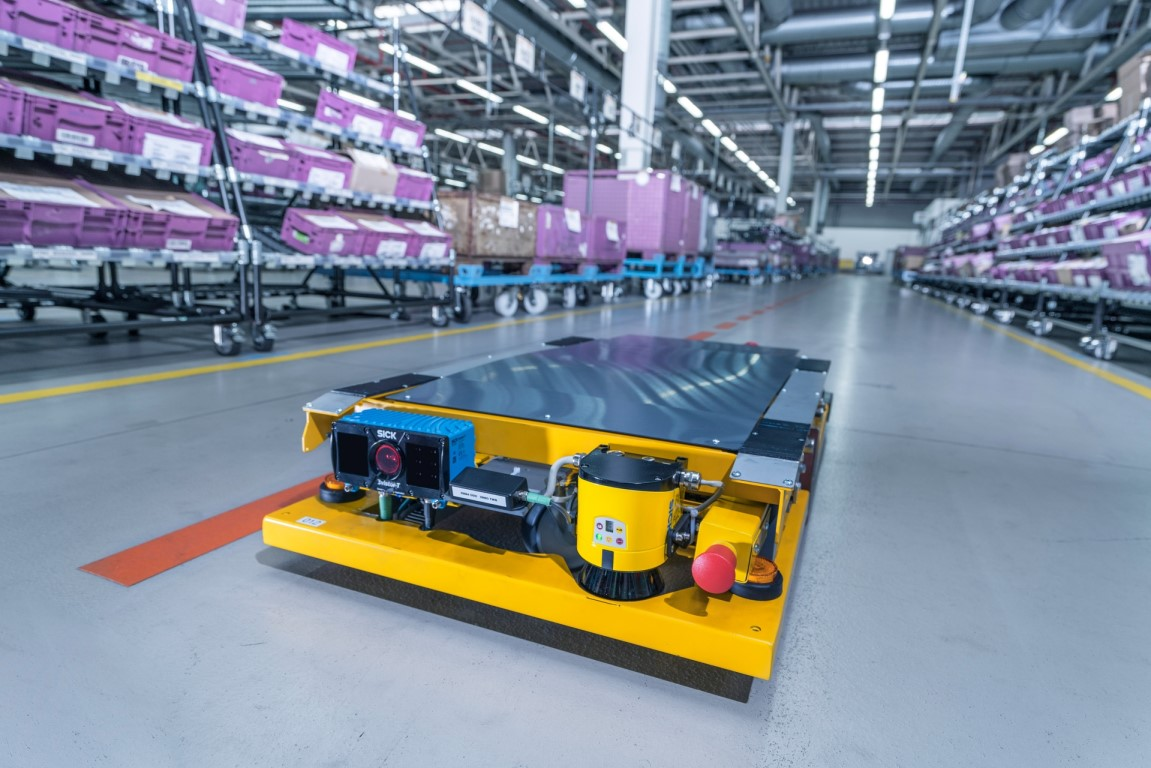
\includegraphics[width=9cm]{figures/bmw.jpg}
	\label{bmw}
	\caption{BMW: Smart Transport Robots}
\end{figure}

A company, named AETHON, made fully autonomous robot called TUG that automates the transport of materials and supplies in commercial environments. It can automatically drop off and pickup of carts, navigates on internal map of facility using laser and it has a omnidirectional 4 wheel driven drive system for higher maneuverability.

\begin{figure}[htb!]
	\centering
	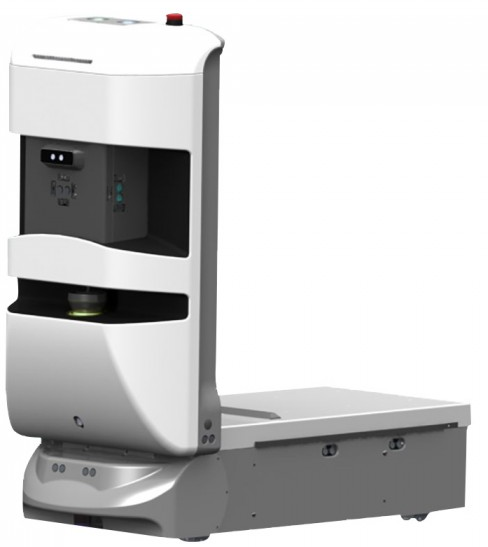
\includegraphics[width=7cm]{figures/tug.png}
	\label{bmw}
	\caption{AETHON: TUG mobile transport robot}
\end{figure}

Another interesting field of application of transportation robots is the military. By putting humans to this work they are often exposed to a risk that could be avoided.The Autonomous Platform Demonstrator is a military transportation robot developed by the U.S. It has a hybrid-electric drive train with six in-hub electric motors powered by li-ion batteries charged using an on-board diesel generator. 

\begin{figure}[h]
	\centering
	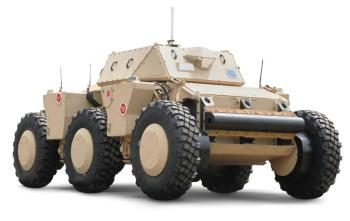
\includegraphics[width=7cm]{figures/apd.jpg}
	\label{bmw}
	\caption{Military transportation robot: APD}
\end{figure}

From control point of view it can be controlled in real-time by a soldier or it can operate autonomously. Autonomously it can operate at speeds up to 50 mph. It can travel along a GPS way point route and avoid obstacles in its way. \cite{apd}






\newpage

\section{Mobile Robots}
The general platform of the transportation robots is obviously the family of mobile robots. Generally a mobile robot faces more design challenges compared to robots that operates in fixed positions as it is left alone in the world. The most critical design problem is related to the locomotion which has to be suited with the conditions of the given ground. In order to handle the changes of the environment and to be able to make decisions during runtime as function of actual state, the robots need to have more intelligence and self-determination. The mobile robots are still not reliable enough nowadays to operate in wide ranges outside of laboratory walls. They need to have a built-in model about their environment, furthermore they need to detect and analyse that of changes and their actual positions have to be found in order to be able to design and perform the next movements. In other words, a sequence of intelligent acts are expected to carry out based on interactions with the dynamically changing outside world.
\subsection{Classification of mobile robots}
\subsubsection{Based on the medium in which the robot moves}
\begin{itemize}
	\item \textbf{Air/Space} \\
		These are mostly applied in space flight and military. The most well known application is the Unmanned Aerial Vehicles (UAV), commonly known as drone, which is an aircraft without pilot. The drones develop fast as they are easier to build and control as they do not have to navigate between obstacles.
	\item \textbf{Water} \\
		Automated Underwater Vehicles (AUV) are generally used in seas and oceans for research and industrial purposes. One of the most interesting field is the development of amphibious vehicle that can operate either on earth or on water.
	\item \textbf{Earth} \\
		As it is our natural habitat, the robots operating on earth are the most common.	
\end{itemize}
\subsubsection{Based on the locomotion mechanism}
Mobile robots generally locomote either using wheeled mechanism, a well-known human technology for vehicles, or using a small number of articulated legs being inspired by biological systems. In general, legged locomotion requires higher degrees of freedom and therefore greater mechanical complexity than wheeled locomotion. Wheels, in addition to being simple, are extremely well suited to flat and hard ground, thus their energy need is radically less compared to legged locomotion. However, the softer the surface, the higher the rolling friction which results a dramatic efficiency loss in case of wheeled robots. The efficiency of wheeled locomotion depends on the flatness and hardness of the ground, while the efficiency of legged locomotion depends on the leg mass and body mass. The nature prefers the legged locomotion since they must operate on rough and unstructured terrain where a wheeled vehicle could get stuck easily, e.g. in the case of Sojourner Mars rover in 1997. They are simply unable to step over an obstacle, the only chance is to avoid it.
On the other hand, it is also understandable the most of the industrial applications of mobile robotics utilize some form of wheeled locomotion due to the fact that the human environment mostly consists of smooth surfaces, both indoors and outdoors. In such conditions, the wheeled configurations are currently faster and more mobile.

In locomotion, the environment is fixed and the robot moves by imparting force to the environment. The scientific basis is the study of actuators that generate interaction forces and mechanisms that implement the desired kinematic and dynamic properties. The core issues that are need to be evaluated to analyse a robot configuration in terms of locomotion are the followings:
\begin{itemize}
	\item Stability
		\begin{itemize}
			\item number and geometry of contact points
			\item center of gravity
			\item static/dynamic stability
			\item inclination of terrain
		\end{itemize}
	\item Characteristics of contact
		\begin{itemize}
			\item contact point/path size and shape
			\item angle of contact
			\item friction
		\end{itemize}
	\item Type of environment
	\begin{itemize}
		\item structure
		\item medium, (e.g. water, air, soft or hard ground)
	\end{itemize}

\end{itemize}


\subsection{Legged Mobile Robots}
Legged mobile robots contact the ground by a set of contact points which provides good adaptability and maneuverability in rough terrain. Not even the ground quality is an issue until the ground clearance is possible to be maintained, e.g crossing holes which does not exceed the size of the robot is solvable demand. The main disadvantages of legged systems include power and mechanical complexity. The leg must be capable of sustaining the part of the robot’s total weight, lifting and lowering the robot body meanwhile keeping the stability permanently. Furthermore, high maneuverability needs sufficient number of degrees of freedom to impart forces in a sufficient number of different directions.
The legged robots are basically biologically inspired based on the fact that they are successful locomotion systems. A number of different leg configurations have been successful in a variety of organisms, i.e. the most common numbers are the two, four or six.

\begin{figure}[h]
	\centering
	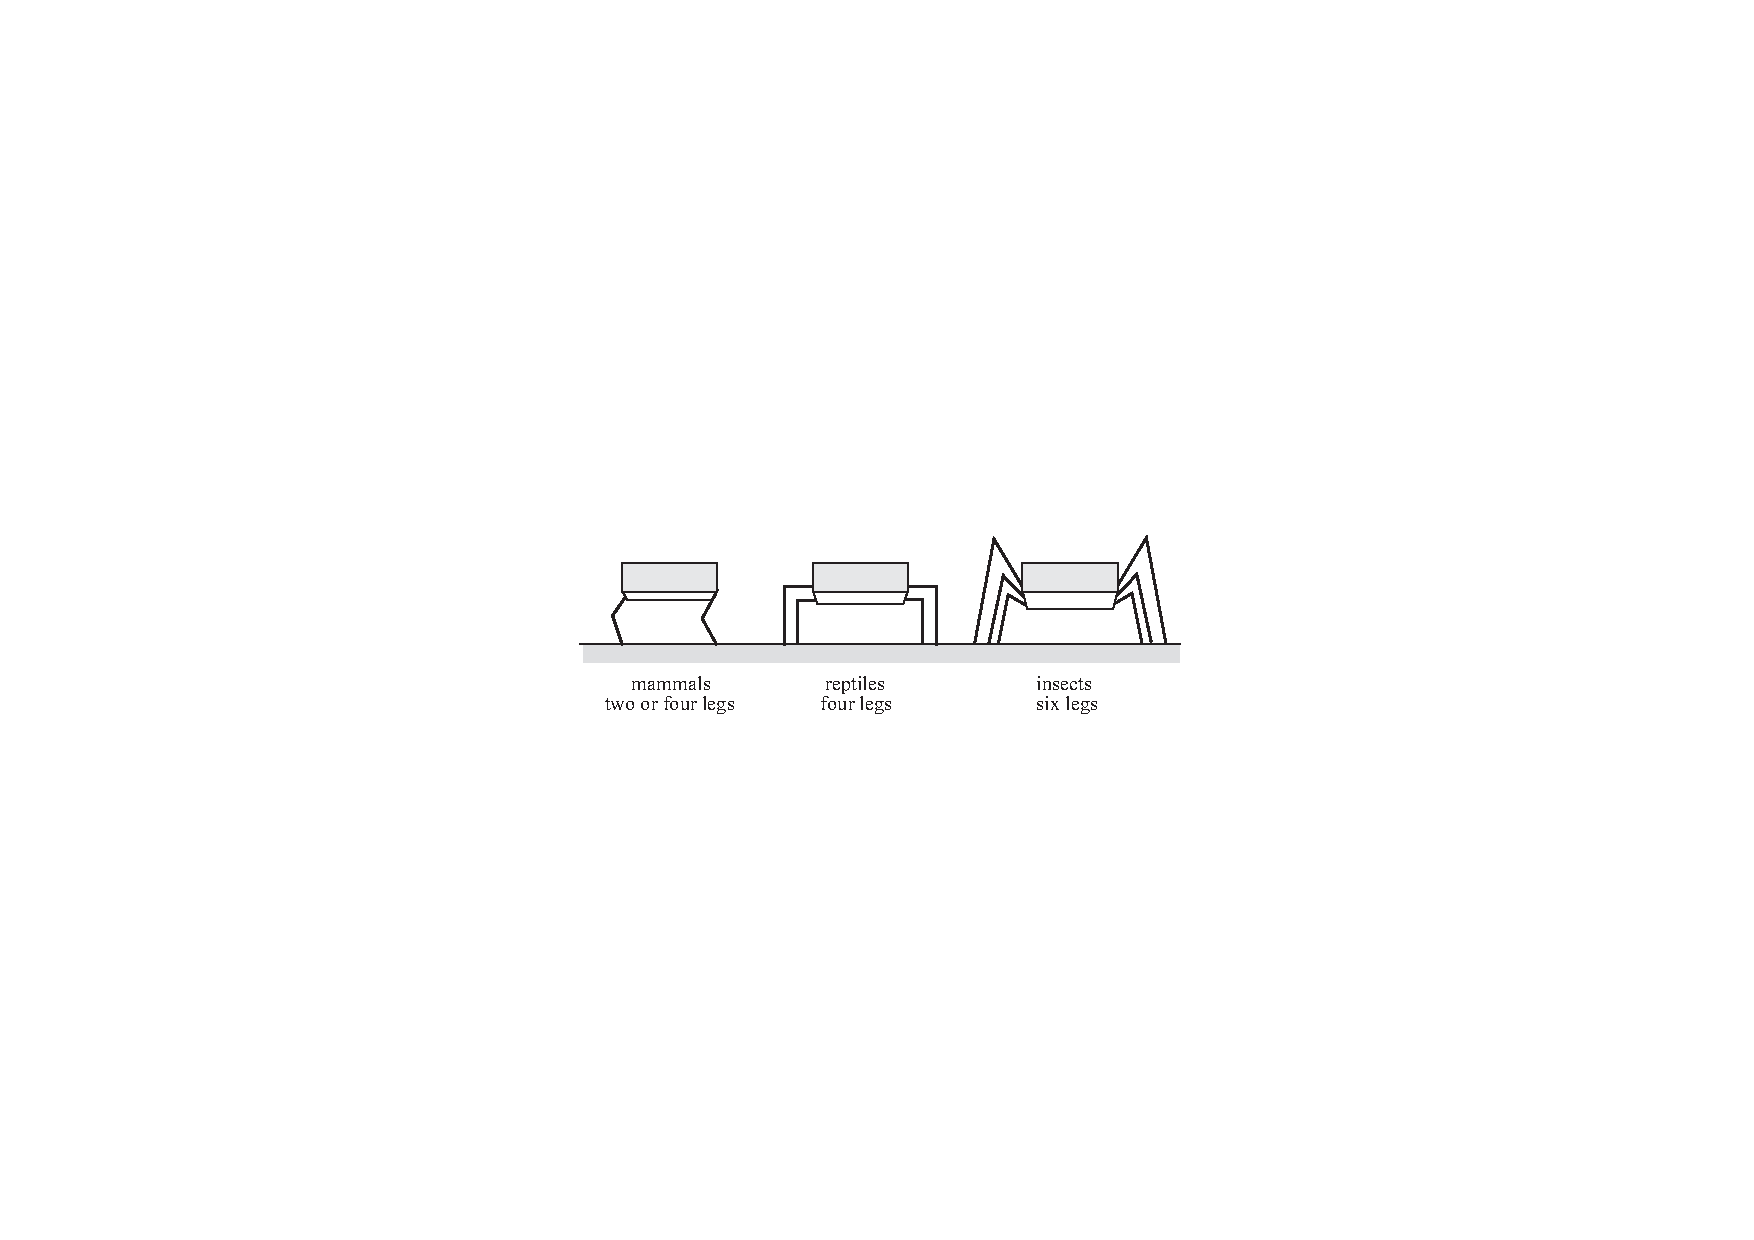
\includegraphics[width=7cm]{figures/legged2.pdf}
	\label{legged}
	\caption{Arrangement of the legs of various animals}
\end{figure}

A creature with at least three legs can achieve static balance which means that no correcting movements have to be taken to preserve its balance. Actually static balance means that the center of gravity is within the tripod of ground contact. A small deviation from stability is passively corrected toward the stable pose by constrain forces after the disturbance goes away. However, any creature who is intended to walk must be able to lift and then release their legs, thus for static walking the minimum number of needed legs is six. Insects and spiders are immediately able to walk when born compared to mammals with four legs who are not able to walk or even to stand in case of humans with only two legs. Therefore the main issue regarding the locomotion of legged robots is the balancing. Of course, the number of legs and also the number of degrees of freedom of a given leg can be increased in order to achieve better stability and maneuverability. On the other hand, more legs and joints result more actuators, thus more energy, more mass, more control, i.e. more costs in certain senses. Most of the legged robots in research and industrial cases have two legs.
The robot legs and arms are usually driven by electrical motors and pneumatic pistons. High level of harmony of the piston movements must be carried out by the designer in order to its hold balance also during the walking what is challenging control task.

\subsection{Wheeled Mobile Robots}
The wheels are the most widely used locomotion mechanisms in man-made vehicles in general due to its simplicity, effectiveness. In most of the cases, during the design the robot builders need to focus problems regarding traction, stability, maneuverability and control. 

\begin{figure}[h]
	\centering
	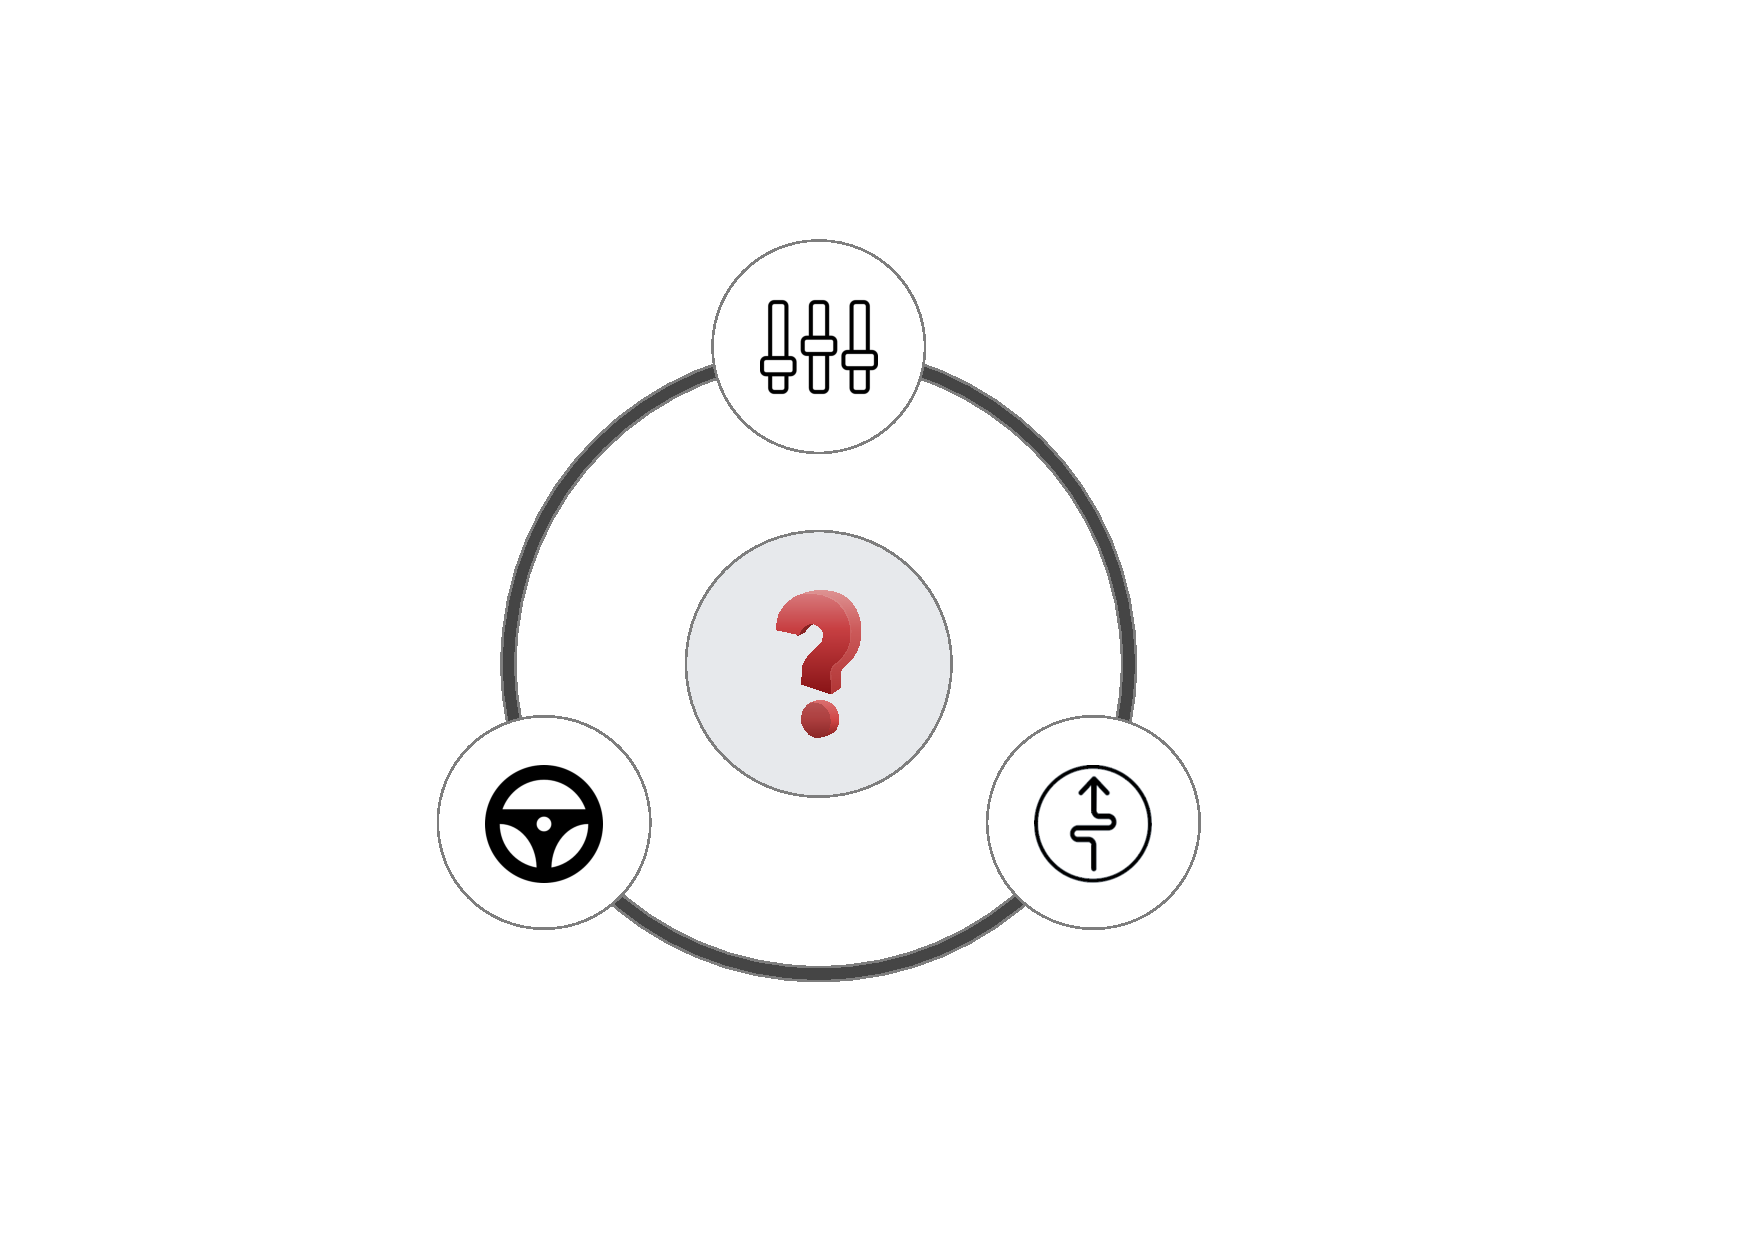
\includegraphics[width=4cm]{figures/triangle.pdf}
	\label{triangle}
	\caption{Major aspects of wheeled robot design}
\end{figure}

In general, balance is not usually an issue in wheeled robotics as they are designed such a way that the all wheels are in contact with the ground. Having three wheels is sufficient to guarantee the static stability if the center of gravity is within the triangle formed by three contact points. Obviously in case of two wheels, self-balancing is necessary. When more than two wheels are used, once the stability improved by adding more contact possibilites, but also a flexible suspension system is required to allow all wheels to maintain ground contact when the robot encounters uneven terrain. One of the simplest approaches to suspension is to design flexibility into the wheel itself, i.e. applying deformable tire of soft rubber material.

Basically, the maneuverability of a given robot depend on the design, the configuration and the degrees of freedoms of powered wheels. Each configuration, wheels type has their advantages and disadvantages that have to be considered before building a mobile robot, we shall see the details later. The robot arrangements can be classified into two groups: holonomic and anholonomic. A mechanical system is called anholonomic if in a specific configuration (state) there exists such displacement or rotation that cannot be carried out by means of the combination of possible actuators. A well known example, an automobile cannot move perpendicular to its orientation because of the kinematic constrains of the wheels. On the other hand, some robots are holonomic, in other words omnidirectional, meaning that they can move at any time in any direction along the ground plane (x,y) regardless of the orientation of the robot around its vertical axis. This level of maneuverability requires wheels that can move in more than just one direction, we shall see the detauls later too.

There is generally an inverse correlation between controllability and maneuverability. For example, the omnidirectional designs require significant processing to convert desired rotational and translational velocities to individual
wheel commands. Furthermore, such omnidirectional designs often have greater degrees of freedom at the wheel. Controlling an omnidirectional robot for a specific direction of travel is also more difficult and often less accurate when compared to less maneuverable designs.

As conclusion, there is no perfect robot configuration that simultaneously maximizes stability, maneuverability, and controllability. For that reason, it is always the designer's task to choose the most appropriate mobile robot configuration considering the constraints originated from the given application.


\subsubsection{Wheel design}
The choice of the wheel type has a large effect on the overall kinematics. There are four major wheel classes as shown in the figure below.
\begin{figure}[h]
	\centering
	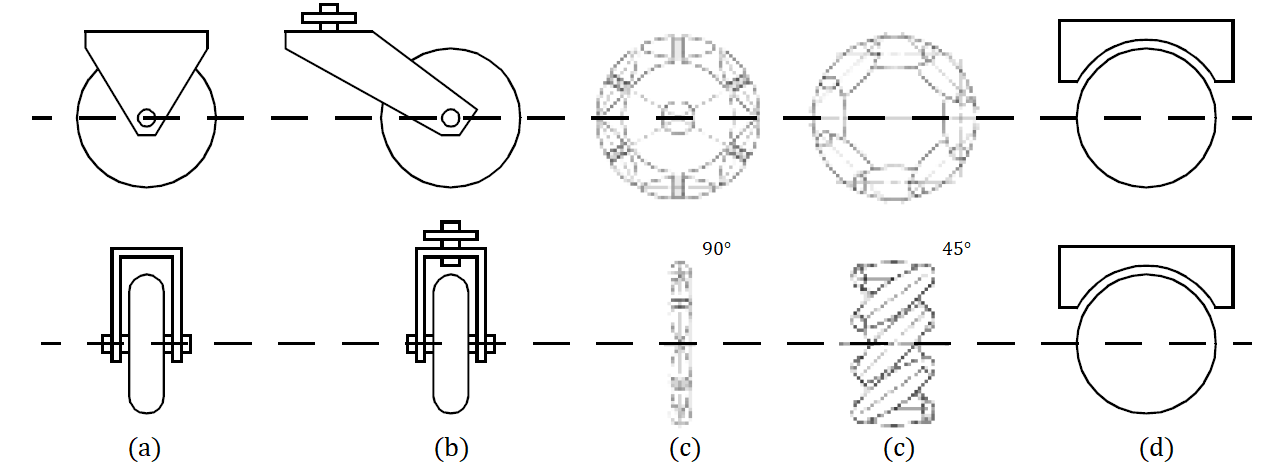
\includegraphics[width=7cm]{figures/wheels4.png}
	\label{wheels}
	\caption{Major classes of wheels: 
		(a) Standard wheel, (b) Castor wheel, (c) Swedish wheel (45$^{\circ}$/90$^{\circ}$), (d) Ball wheel}
\end{figure}
The standard and castor wheel have are highly one-directional as they have a primary axix around they can rotate. These wheels must be steered along a vertical axes to move in a different direction. The main difference between the two configuration is that the castor wheel rotates around an offset vertical axes causing adverse force imparted to the case compared to the standard wheel case where the axes of rotation passes through the contact point. Both the Sweedish and the spherical wheel are less directionally constrained than the former conventional ones. The Swedish wheels functions such as normals wheels providing low resistance in another direction as well, i.e. rolling resistance instead of sticking. Small rollers are attached around the circumference can rotate only in a passive way while the primary axes are the only powered joints. As a result, although the wheel can be driven along only one principal axis, the wheel can move along almost any trajectory. The spherical wheel is a truly omnidirectional wheel, often designed so that it may be actively powered to spin along any direction.

\subsubsection{Wheel configurations}
\paragraph{Holonomic robots}
In practical applications, holonomic systems are rarely present due to higher prices and mechanical complexity, moreover dead reckoning by means of odometry is quite inaccurate. \\[10pt]
\noindent \textbf{Three wheeled omnidirectional mobile robot} \\
The mechanically simplest holonomic robot is omnidirectional configuration. At least three independently driven wheels are needed to be able to move in any direction $(x,y,\varphi)$ in ground plane at any time.
\begin{figure}[htb!]
	\centering
	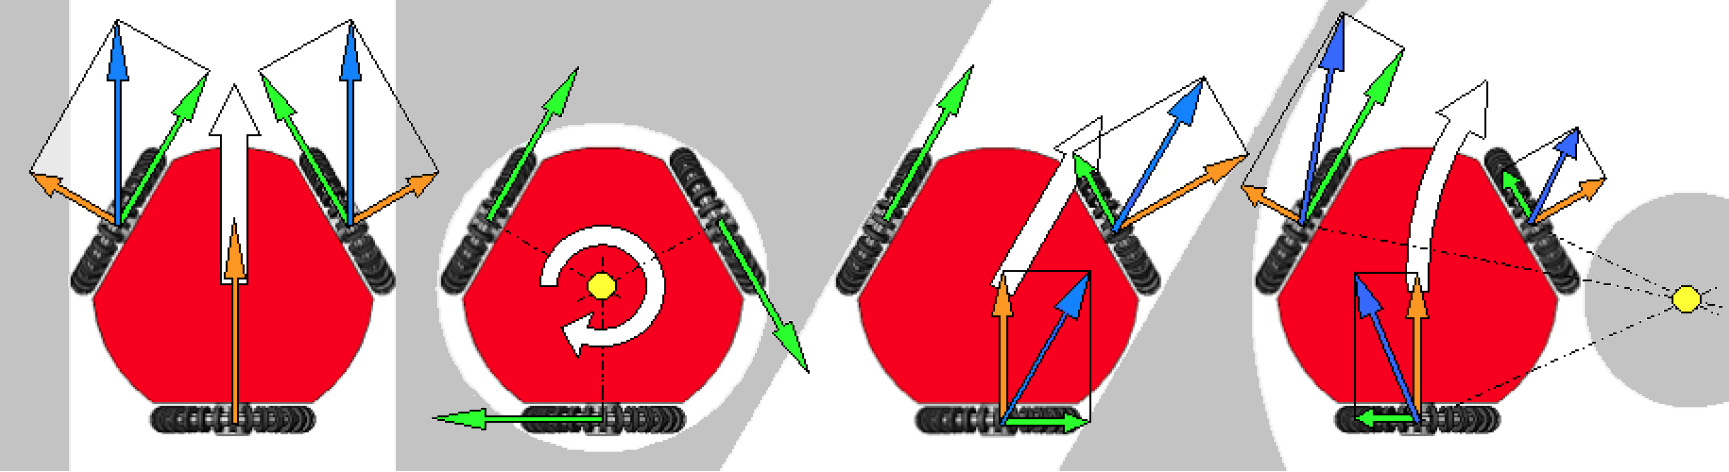
\includegraphics[width=10cm]{figures/omniconfig.png}
	\caption{Three-wheeled omnidirectional drive configuration}
	\label{omniconfig}
\end{figure}
The resultant velocity vectors in terms of wheel velocities can be seen in Figure \ref{omniconfig}. The blue wheel velocity vectors can have lateral component, i.e. the wheels have to be able to move parallel to their primary axes. This kind of configuration needs the previously mentioned Swedish wheels or spherical wheels. 
In addition, also four wheels or even more can be built-in in a system, but in this case it can occur that the wheels drive each other in reverse direction, furthermore the more than three contact point does not guarantee the proper contact of each wheels with the ground.\\[10pt]
\noindent \textbf{Omnidirectional robot with four Swedish wheel} \\
Four-wheeled arrangement with 45$^{\circ}$ Swedish wheels, each driven by a separate motor, have been used in several research and industrial projects. A good example is is Uranus that can rotate and translate independently without any constraints by means of omnidirectional wheels.
\begin{figure}[htb!]
	\centering
	\minipage{0.47\textwidth}
	\centering
	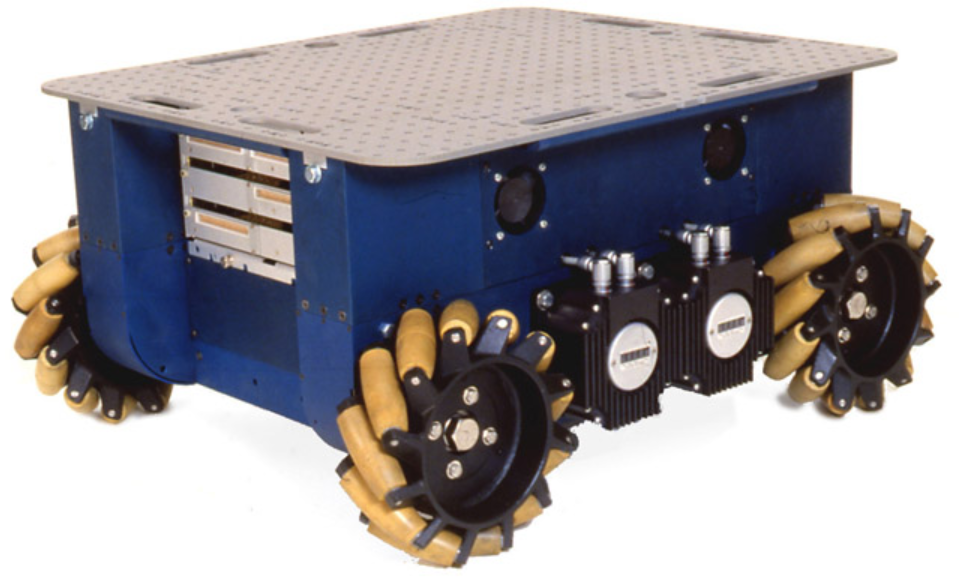
\includegraphics[height=3cm]{figures/uranus}
	\caption{Carnegie Mellon Uranus robot}
	\endminipage\hfill
	\minipage{0.53\textwidth}
	\centering
	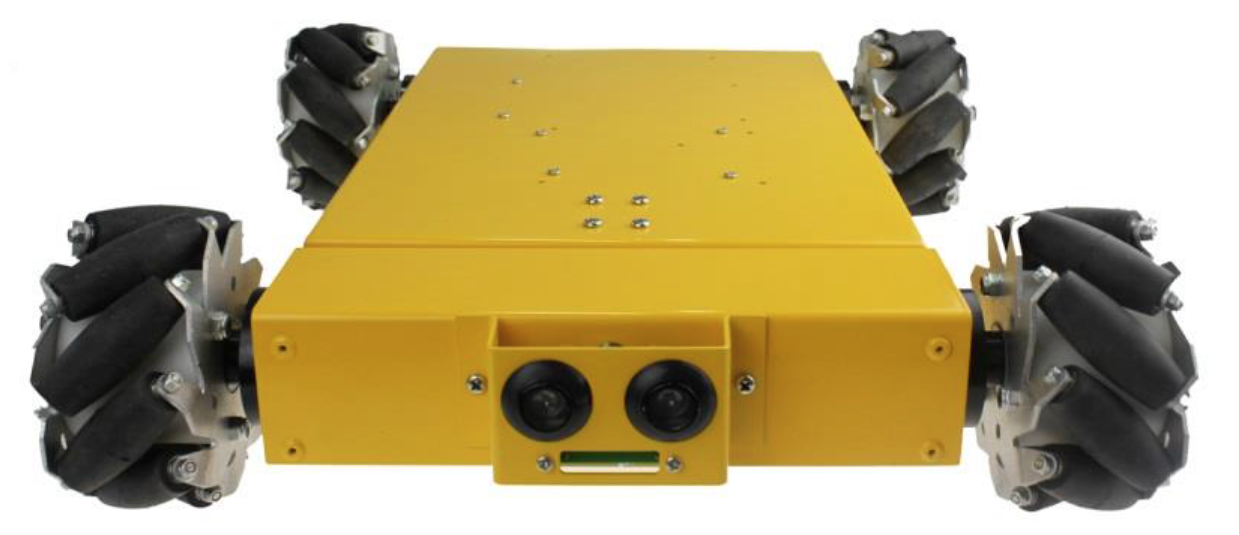
\includegraphics[height=3cm]{figures/mecanum}
	\caption{Mecanum AB robot}
	\label{conv2}
	\endminipage\hfill
\end{figure} \\
When all four wheels spin in the same direction, the robot moves longitudinally in a straight line forward or backward, accordingly. When one diagonal pair of wheels spin in the same direction and the other diagonal pair of wheels spin in the opposite direction, the robot moves purely laterally. The simultaneous spin can be achieved if the wheels on left side are driven in forward or backward while the wheels on the other side are driven the corresponding opposite direction. As it was discussed earlier, this four-wheel arrangement is not minimal in terms of control, stability and maneuverability, but prefered over three-wheeled configuration for higher capacity and stability reasons. \\[10pt]
Main disadvantages of omnidirectional configurations includes the complexity of control because of the more complex processing of wheel velocities. For instance, the Swedish wheels has a set of free rollers along the wheel perimeter adding extra degrees of freedom,i.e. translation in the lateral direction. Furthermore, due to these rollers the wheel perimeter is not a perfect circle, thus accuracy of dead-reckoning based on counting the number of rotations might be inaccurate soon. The rollers can also cause slippage, thus accumulation of displacement errors.

\paragraph{Anholonomic robots}















%%%%%%%%%%%%%%%%%%%%%%%%%%%%%%%%%%%%%%%%%%%%%%%%%%%%%%%%%%%%%%%%%%%%%%%%%%%%%%%%%%%%%%%%%%%%%%%%%%%%%%%%%%%%
% 											Bibliography
%%%%%%%%%%%%%%%%%%%%%%%%%%%%%%%%%%%%%%%%%%%%%%%%%%%%%%%%%%%%%%%%%%%%%%%%%%%%%%%%%%%%%%%%%%%%%%%%%%%%%%%%%%%%

\newpage
\begin{thebibliography}{1}

\addcontentsline{toc}{section}{References}

\bibitem {c} 
James M. Anderson, Nidhi Kalra, Karlyn D. Stanley, Paul Sorensen, Constantine Samaras, Oluwatobi A. Oluwatola: \emph{Autonomous Vehicle Technology}

\bibitem {5c} 
http://iiot-world.com/artificial-intelligence/five-challenges-in-designing-a-fully-autonomous-system-for-driverless-cars/

\bibitem {smp} 
SMP Robotics: https://smprobotics.com/ \href{https://smprobotics.com/application_autonomus_mobile_robots/transport-robots/}{[link]}

\bibitem {starship} 
Starship Technologies: https://www.starship.xyz/ \href{https://www.starship.xyz/}{[link]}

\bibitem {neo} 
NEOBOTIX: https://http://www.neobotix-robots.com/ \href{http://www.neobotix-robots.com/}{[link]}

\bibitem {bmw} 
BMW STR: http://www.bmwblog.com/ \href{http://www.bmwblog.com/2016/11/18/bmw-logistics-now-use-autonomous-transport-robots/}{[link]}

\bibitem {apd} 
Allonrobots: http://www.allonrobots.com/military-transportation-robots.html \href{http://www.allonrobots.com/military-transportation-robots.html}{[link]}



\bibitem{whatisarduino} Alan G. Smith: \emph{Introduction to Arduino, 2011}


\bibitem{communication_arduino} Brian W. Evans: \emph{Arduino Programming Notebook, 2007}


\bibitem{i2c_communication_arduino} Alex Lange: \emph{I2C Communication with Arduino, 2015}

\bibitem{i2C_communication_arduino_2} http://howtomechatronics.com \href{http://howtomechatronics.com/}{[link]}

	\bibitem{orientation_arduino} Kevin Townsend: \emph{Adafruit BNO055 Absolute Orientation Sensor, 2017}

	\bibitem{optical flow} https://github.com/Lauszus/ADNS3080 \href{https://github.com/Lauszus/ADNS3080}{[link]}
	
\end{thebibliography}

\end{document}
